% -*- TeX -*- -*- UK -*- -*- BMR -*-
% ----------------------------------------------------------------
% Beamer presentation ************************************************
% **** -----------------------------------------------------------
\documentclass{beamer}%[handout][hyperref={backref=slide}]

\usepackage{array}
\usepackage{cancel}
%\input{sl_slide_preamble.tex}
\input{sl_slide_preamble_nonotes.tex}
%\usecolortheme[named=darkblue]{structure}
\usecolortheme[rgb={0.6372549 0.27843137 0.27058824}]{structure}
\setbeamercolor{alerted text}{fg=red!80!black}
\input{sl_slide_graphics_preamble.tex}
\input{sl_definitions.tex}
\input{sl_slide_symbols.tex}
%
\graphicspath{{"Figs/"}}
\DeclareMathOperator{\SNR}{SNR}
\DeclareMathOperator{\snr}{SNR}
%matrices
\newcommand{\inv}{^{-1}}
\newcommand{\I}{\mathbf{I}}
%prob vector
\newcommand{\pr}{\mathbf{p}}
%equilibrium distribution
\newcommand{\eq}{\pr^\infty}
%first passage times
\newcommand{\fpt}{\mathbf{T}}
%off-diag first passage times
\newcommand{\fptb}{\overline{\fpt}}
%other symbols
\newcommand{\w}{\mathbf{w}}
\newcommand{\W}{\mathbf{W}}
\newcommand{\frg}{\W^\mathrm{F}}
\newcommand{\M}{\mathbf{M}}
\newcommand{\F}{\boldsymbol{\Phi}}
\newcommand{\wv}{\vec{w}}
%super/subscripts
\newcommand{\pot}{^{\text{pot}}}
\newcommand{\dep}{^{\text{dep}}}
\newcommand{\potdep}{^{\text{pot/dep}}}
\newcommand{\lmax}{_{\text{max}}}
\newcommand{\lmin}{_{\text{min}}}
%quantities
\newcommand{\initial}{\mathcal{I}}
\newcommand{\area}{\mathcal{A}}
\newcommand{\CS}{\mathcal{S}}
\newcommand{\comp}{^\mathrm{c}}
\renewcommand{\e}{\mathsf{e}}
%---------Title-----------------------------------------------------------

\title[Impaired/enhanced learning w/ enhanced plasticity]{Modelling impaired  and enhanced learning with enhanced plasticity}
%
%\subtitle{\small{based on work with: Barbara Nguyen-Vu, Grace Zhao, Aparna Suvrathan, Han-Mi Lee, Surya Ganguli, Carla Shatz and Jennifer Raymond
%}}
%
\author[S.~Lahiri et al.]{Subhaneil Lahiri \\ with: Barbara Nguyen-Vu, Grace Zhao, Aparna Suvrathan, Han-Mi Lee, Surya Ganguli, Carla Shatz and Jennifer Raymond%\inst{1}
}
%
\institute[Stanford]{%
%\inst{1}
Stanford University
}
%
\date{December 3, 2014}
%
%\slideCaption{}

%---------Beginning--------------------------------------------------------

\begin{document}

%-------------Slide--------------------------------------------------------

\begin{frame}
%
 \titlepage

 \vspace{-1cm}
 \parbox[t]{0.3\linewidth}{
 \begin{center}
 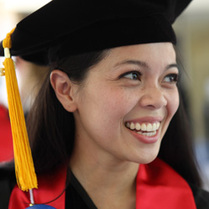
\includegraphics[height=0.55\linewidth]{barbara.jpg}\\
 \small Barbara Nguyen-Vu
 \end{center}
 }
 \hfill
 \parbox[t]{0.3\linewidth}{
 \begin{center}
 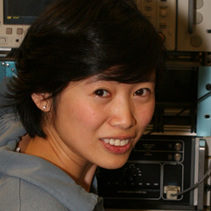
\includegraphics[height=0.55\linewidth]{grace.jpg}\\
 \small Grace Zhao
 \end{center}
 }
 \note[item]{Acknowledge Barbara and Grace}
%
\end{frame}

%-------------Slide--------------------------------------------------------

\begin{frame}{Introduction}
%
\parbox[t]{0.69\linewidth}{%
 Learning requires synaptic plasticity.\\
 Expect: enhanced plasticity \lto\ enhanced learning.
}
\parbox[t]{0.29\linewidth}{%
 \hfill{\alignmid{
\includegraphics[width=0.4\linewidth]{the_brain_by_lonewolf16.jpg}}}
}
 \\
 \citerr{Tang1999enhancedLearning,Malleret2001enhancedLearning,Guan2009enhancedLearning}\\
 \note[item]{It does help in some cases}
\onslide<2->
\parbox[t]{0.69\linewidth}{%
 But often: enhanced plasticity \lto\ impaired learning.
}
\parbox[t]{0.29\linewidth}{%
 \hfill{\alignmid{
\includegraphics[width=0.4\linewidth]{pinky_by_lonewolf16.jpg}}}
}
 \\
 \citerr{Migaud1998impairedLearning,Uetani2000impairedLearning,Hayashi2004impairedConsolidation}\\
 \citerr{Cox2003impairedLearning,Rutten2008impairedLearning,Koekkoek2005impairedConditioning}\\
 \note[item]{Want to understand when and why}

 \onslide<3->\vp Mice with enhanced cerebellar plasticity can show \alert{both} impaired and enhanced learning.
 \note[item]{Depends on circumstance. Rich pattern of behaviour}

 \vp Simple synapses \alert{cannot} explain behaviour.
 \alert{Complex synapses} are required.\\
 \lto\ predictions for synaptic physiology.
 \note[item]{Develop understanding of when and why learning is enhanced/impaired}
%
\end{frame}

%%-------------Slide--------------------------------------------------------
%
%\begin{frame}{Outline}
%%
% %\tableofcontents[hideallsubsections]
% \begin{itemize}
%   \item Motor learning
% \begin{itemize}
%   \vp\item Cerebellar learning of mice with enhanced plasticity
%
%   \vp\item Complex synaptic models
% \end{itemize}
%   \vp\item (Memory capacity of complex synapses)
% \end{itemize}
% %
%%
%\end{frame}
%
%%%-------------Section--------------------------------------------------------
%%
%%\section{VOR learning and the cerebellum}
%%
%-------------Slide--------------------------------------------------------

\begin{frame}{Vestibulo-Occular Reflex}
%
 \parbox[t]{0.35\linewidth}{\aligntop{
\includegraphics[width=0.99\linewidth]{VOR.svg}}}
 \parbox[t]{0.64\linewidth}{%
 Eye movements compensate for head movements $\implies$ stabilise image on retina.

 \vp Requires control of $\text{VOR gain} = \frac{\text{eye velocity}}{\text{head velocity}}$.

 \vp Needs to be adjusted as eye muscles age, \etc
 }

%
\end{frame}


%-------------Slide--------------------------------------------------------

\begin{frame}{Vestibulo-Occular Reflex training}
%
\note[item]{Explain what VOR gain is}
 \parbox[t]{0.2\linewidth}{%
   \aligntop{
\includegraphics[width=0.99\linewidth]{VORinc.svg}}
     \note[item]{trick brain into thinking VOR gain needs adjusting my moving visual stimulus}
     \note[item]{anti-phase \lto\ increase gain}

   \vp\aligntop{
\includegraphics[width=0.99\linewidth]{VORdec.svg}}
     \note[item]{in phase \lto\ decrease gain}
   }
 \hspace{0.15\linewidth}
 \parbox[t]{0.59\linewidth}{%
 \raggedleft
   \aligntop{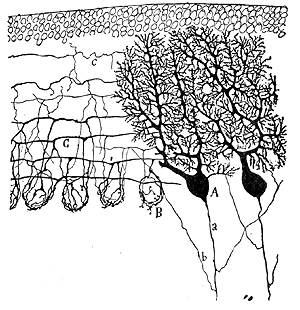
\includegraphics[width=0.5\linewidth]{pk.png}}\\
   \rref{Cajal}

   \vp \begin{tabular}{ll}
   VOR increase: & LTD in PF-Pk synapses.\\
   \end{tabular}

%   \vp  \aligntop{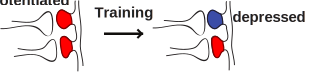
\includegraphics[width=0.8\linewidth]{ltd.svg}}

 }
   \note[item]{Gain change involves cerebellum}
   \note[item]{If we enhanced plasticity here: expect enhanced learning}
%   \note[item]{Marr-Albus-Ito: Pf-Pk synapses}
%   \note[item]{Lisberger-Miles: Vestibular input-VN synapses}
%   \note[item]{Different mechs for different freq, head angle, gain up/down.}
%   \note[item]{Different Pk cells have different tunings.}
%   \note[item]{Gain up in case of interest: LTD in Pf-Pk in flocculus}
%   \note[item]{Gain down: uses different mech for behaviour, but does reverse LTD in Pf-Pk in flocculus}
%   \note[item]{PF-Pk:PF+CF \lto\ LTD, PF+\cancel{CF} \lto\ LTP.}

 \citerr{duLac1995review,Boyden2004review}
%
\end{frame}

%%-------------Section--------------------------------------------------------
%
%\section{The effects of enhanced plasticity and saturation}
%
%-------------Slide--------------------------------------------------------

\begin{frame}{Enhanced plasticity impairs learning}
%
 \alert{Expectation:} enhanced LTD \lto\ enhanced learning.

 \begin{center}
 \begin{tabular}{lr}
%   Baseline & \hspace{0.1\linewidth} &
%   Gain increase \\[0.5cm]
%   \alignmid{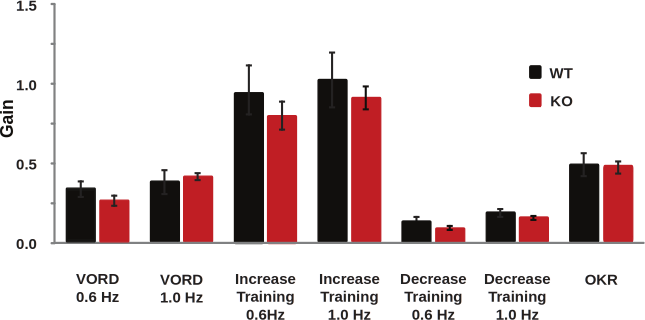
\includegraphics[width=0.4\linewidth]{baseline.svg}} &&
   \alignmid{
\includegraphics[width=0.2\linewidth]{VORinc.svg}}&
   \alignmid{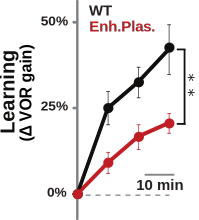
\includegraphics[width=0.3\linewidth]{gain_inc.svg}}\\
   &\alert{Experiment:} enhanced plasticity \lto\ impaired learning.
 \end{tabular}
 \end{center}
% \note[item]{No difference in baseline occulomotor performance}
 \note[item]{Impairment of learning}
 \note[item]{Looking at change of VOR gain during gain-up training}

\vp
 \note[item]{Major Histocompatibility Complex - involved in synaptic plasticity (Carla Shatz lab)}
 Knockout of MHC-I K$^\mathsf{b}$D$^\mathsf{b}$ molecules in PF-Pk synapses\\
  \lto\ lower threshold for LTD  \citerr{McConnell2009MHCcerebellum}


%
\end{frame}

%%-------------Slide--------------------------------------------------------
%
%\begin{frame}{Viral rescue removes defect}
%%
% Local injection of Pk specific virus used to restore the knocked-out molecules.
%
% \vp\begin{center}
%   \alignmid{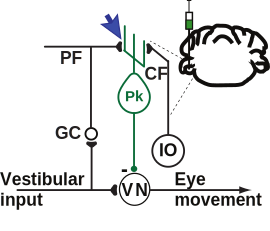
\includegraphics[width=0.3\linewidth]{rescue.svg}}
%   \hspace{0.1\linewidth}
%   \alignmid{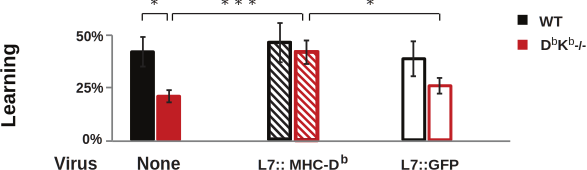
\includegraphics[width=0.5\linewidth]{rescue_results.svg}}
% \end{center}
% \note[item]{removes defect}
% \note[item]{tells us that it is these PF-Pk synapses that are important}
% \note[item]{But what mechanism?}
%%
%\end{frame}
%
%-------------Slide--------------------------------------------------------

\begin{frame}{Depletion hypothesis}
%
{}
 {\color{darkgrey} Learning rate} $\sim$ {\color{darkgreen}intrinsic plasticity rate} $\times$ {\color{darkblue}\# synapses available for LTD}.

 \vp
 \begin{center}

   \parbox[t]{0.25\linewidth}{%\raggedright
     \visible<1,2>{\aligntop{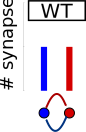
\includegraphics[height=\linewidth]{binary_bar_wt_wo_n.svg}}}
   }
   %
%   \only<1>{\aligntop{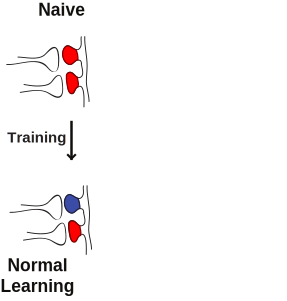
\includegraphics[width=0.3\linewidth]{sat_model_1.svg}}}%
%   \only<2>{\aligntop{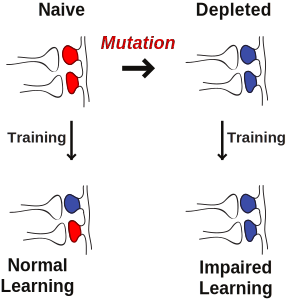
\includegraphics[width=0.3\linewidth]{sat_model_2.svg}}}%
   %
   \hspace{0.3\linewidth}
   %
   \parbox[t]{0.25\linewidth}{%\raggedleft
     \visible<2>{\aligntop{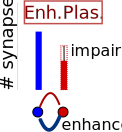
\includegraphics[height=\linewidth]{binary_bar_ko_wo_n.svg}}}
   }

   \vp\visible<2>{\alert{Question 1:} {\color{darkblue}depletion effect} competes with {\color{darkgreen}enhanced intrinsic plasticity}.
   When is depletion effect stronger?}

% \end{tabular}
%   \vp

 \end{center}
% \note[item]{Older explanation: error model}
 \note[item]{Our model: baseline activity \lto\ saturation \lto\ less depression possible}
 \note[item]{Saturation has to compete with enhanced plasticity. Which will win?}
%
\end{frame}

%%%-------------Slide--------------------------------------------------------
%%
%%\begin{frame}{Evidence}
%%%
%% \begin{itemize}
%%   \item Elevated pSer880 - biochemical signature of LTD in region.
%%   \note[item]{predicted by saturation}
%%
%%   \vp \item Local, targeted viral rescue restores WT learning.
%%   \note[item]{must be these synapses}
%%
%%   \vp \item CF stimulation  \lto\ KO learning.
%%   \note[item]{using ChR2 \lto\ saturation by different mechanism}
%% \end{itemize}
%%%
%%\end{frame}
%%
%%-------------Slide--------------------------------------------------------
%
%\begin{frame}{Evidence: level of depression}
%%
% \aligntop{\includegraphics[width=0.3\linewidth]{pSer880.svg}}
% \hp
% \parbox[t]{0.6\linewidth}{%
% Basal level of GluR2 phosphorylation at serine 880 in AMPA receptor.
%
% \vp Biochemical signature of PF-Pk LTD.
%
% \vp Shows that \# depressed synapses in flocculus is larger in KO than WT.
% \note[item]{Predicted by saturation hypothesis}
% }
%%
%\end{frame}
%
%%-------------Slide--------------------------------------------------------
%
%\begin{frame}{Evidence: saturation by CF stimulation}
%%
% Use Channelrhodopsin to stimulate CF \parbox[t]{0.45\linewidth}{%
% \lto\ increase LTD in PF-Pk synapses \\
% \lto\ simulate saturation in WT.
% }
% \note[item]{should result in similar behaviour to KO}
%
% \vp\begin{center}
%   \alignmid{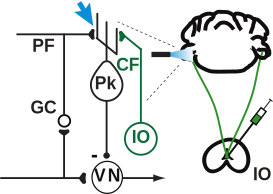
\includegraphics[width=0.4\linewidth]{CFstim.svg}}
%   \hspace{0.1\linewidth}
%   \alignmid{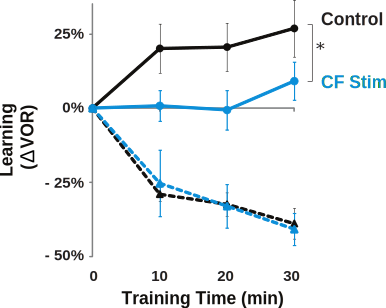
\includegraphics[width=0.4\linewidth]{CFstim_results.svg}}
% \end{center}
%%
%\end{frame}
%
%-------------Slide--------------------------------------------------------

\begin{frame}{Replenishment by reverse-training}
%
 %
 \begin{center}
   \only<1>{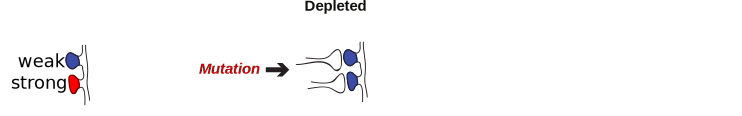
\includegraphics[width=0.7\linewidth]{desat_1.svg}}%
   \only<2>{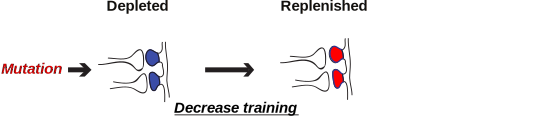
\includegraphics[width=0.7\linewidth]{desat_2.svg}}%
   \only<3->{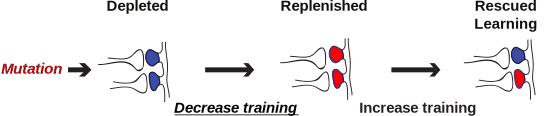
\includegraphics[width=0.7\linewidth]{desat_3.svg}}

   \vp
  \begin{overlayarea}{0.7\linewidth}{0.25\linewidth}
   \only<4>{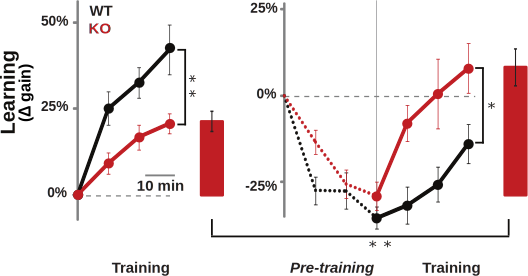
\includegraphics[width=0.9\linewidth]{gain_dec.svg}}%
%
%   \vp
   \only<5->{
   \begin{tabular}{c@{\hspace{0.2\linewidth}}c}
   \color{red!60!black}{Enh.\ Plast.} & WT \\[0.2cm]
   \aligntop{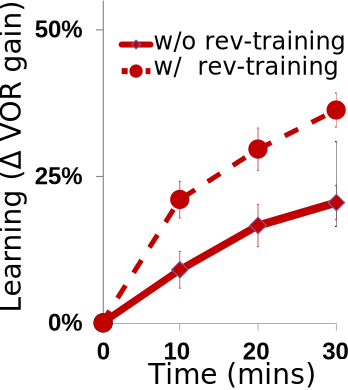
\includegraphics[width=0.35\linewidth]{data_shifted_KO.svg}}
   &
   \aligntop{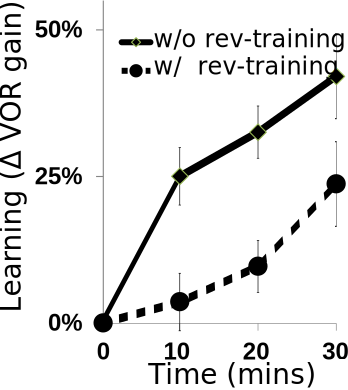
\includegraphics[width=0.35\linewidth]{data_shifted_WT.svg}}
   \end{tabular}
   }
   \end{overlayarea}
 \end{center}

 \visible<5->{\vp\alert{Question 2:} How can replenishment \emph{ever} impair learning?}
 %
 \note[item]{precede gain inc training w/ gain dec rev-training: reverses LTD}
 \note[item]{(but behaviour from elsewhere \lto\ not modelled)}
 \note[item]{Shift origin to compare}
%
\end{frame}


%%-------------Slide--------------------------------------------------------
%
%\begin{frame}{Summary of training results}
%%
% \begin{center}
%   \only<1,6>{\alignmid{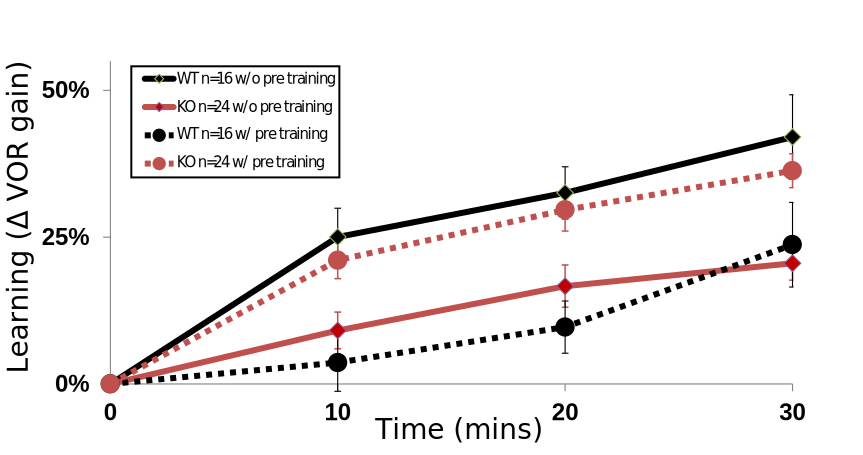
\includegraphics[width=0.29\linewidth]{data_shifted.svg}}}%
%   \only<2>{\alignmid{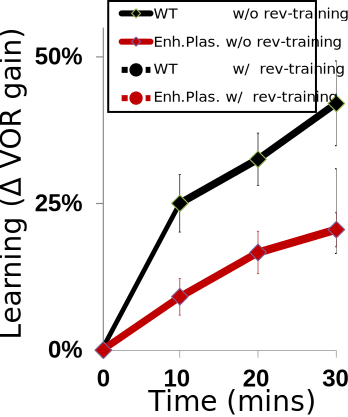
\includegraphics[width=0.29\linewidth]{data_shifted_top.svg}}}%
%   \only<3>{\alignmid{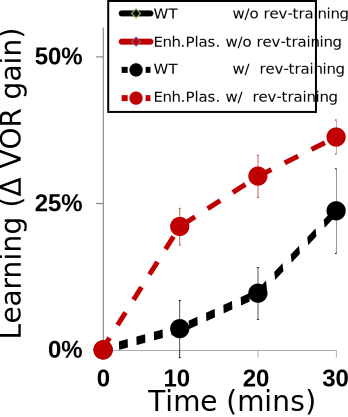
\includegraphics[width=0.29\linewidth]{data_shifted_bottom.svg}}}%
%   \only<4>{\alignmid{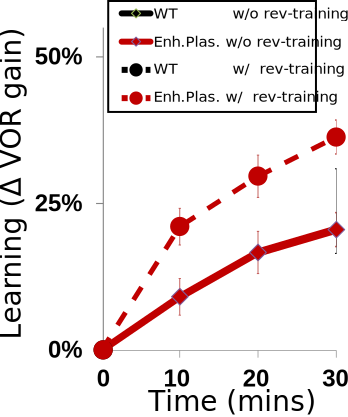
\includegraphics[width=0.29\linewidth]{data_shifted_right.svg}}}%
%   \only<5>{\alignmid{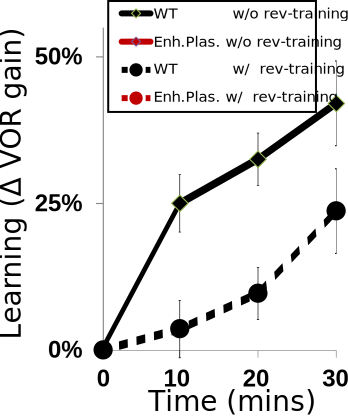
\includegraphics[width=0.29\linewidth]{data_shifted_left.svg}}}
%   \hspace{0.05\linewidth}
%   \only<1>{\alignmid{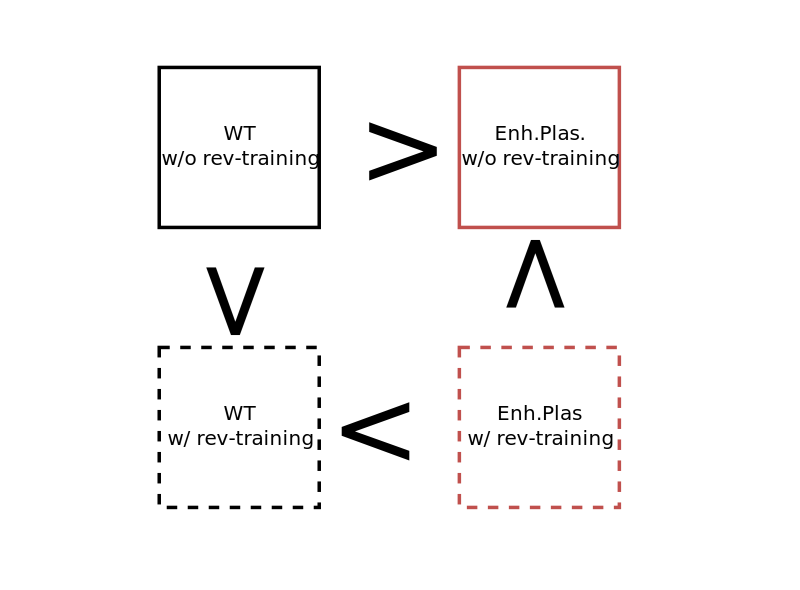
\includegraphics[width=0.55\linewidth]{comparisons_none.svg}}}%
%   \only<2>{\alignmid{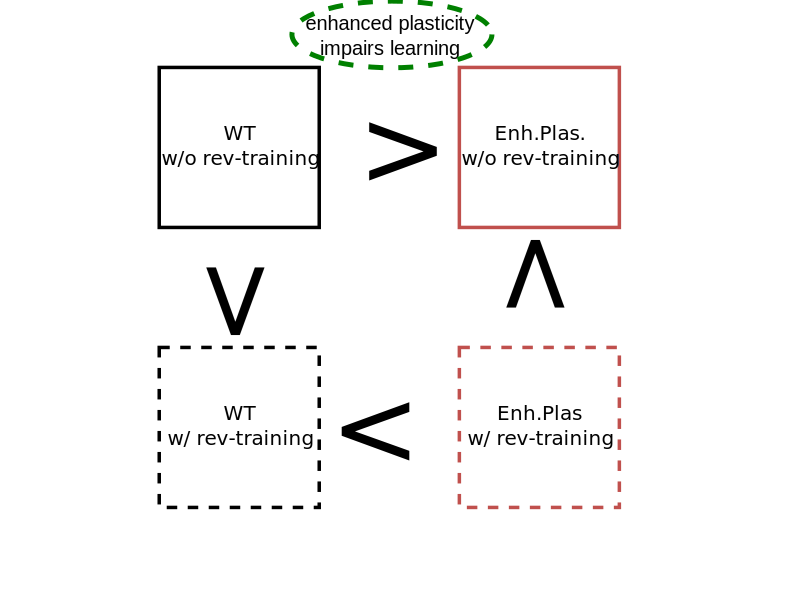
\includegraphics[width=0.55\linewidth]{comparisons_top.svg}}}%
%   \only<3>{\alignmid{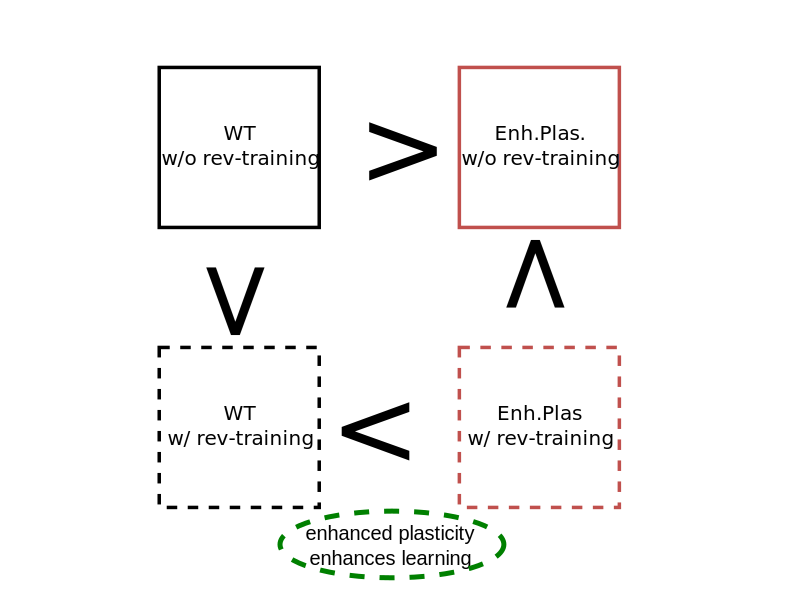
\includegraphics[width=0.55\linewidth]{comparisons_bottom.svg}}}%
%   \only<4>{\alignmid{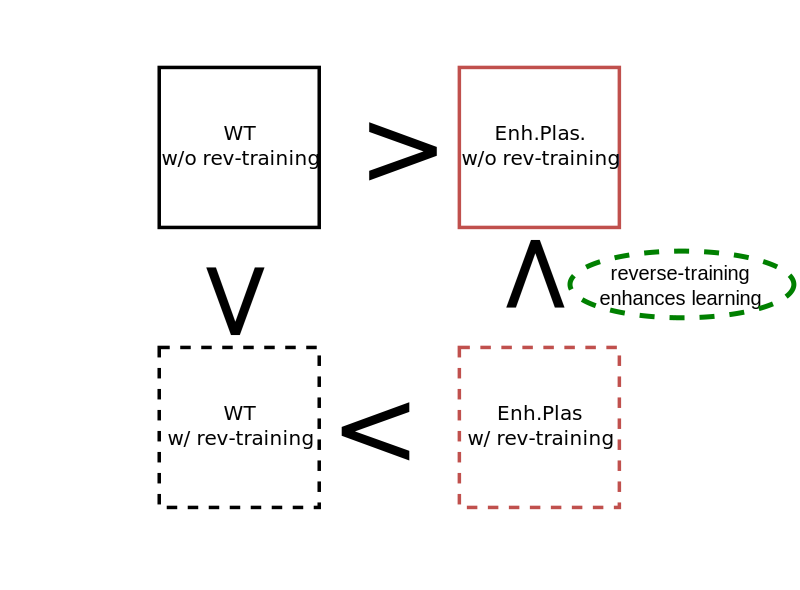
\includegraphics[width=0.55\linewidth]{comparisons_right.svg}}}%
%   \only<5>{\alignmid{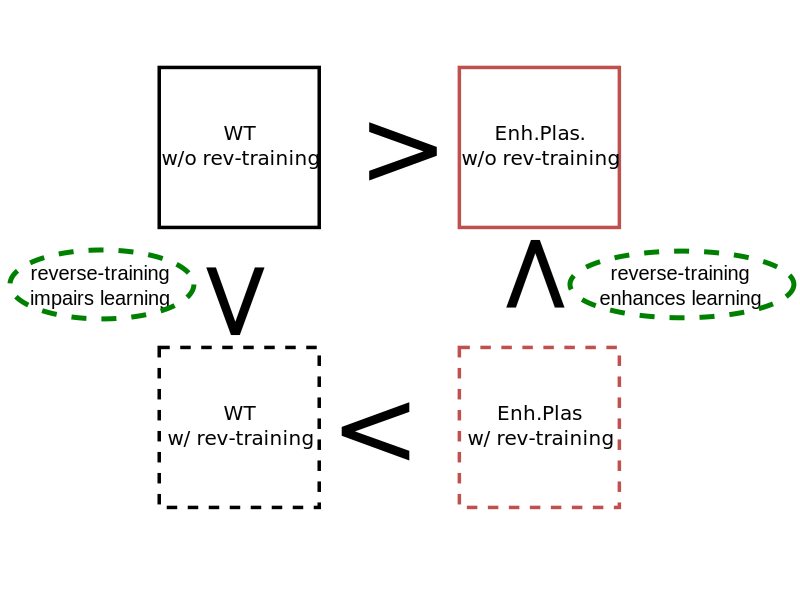
\includegraphics[width=0.55\linewidth]{comparisons_leftright.svg}}}%
%   \only<6>{\alignmid{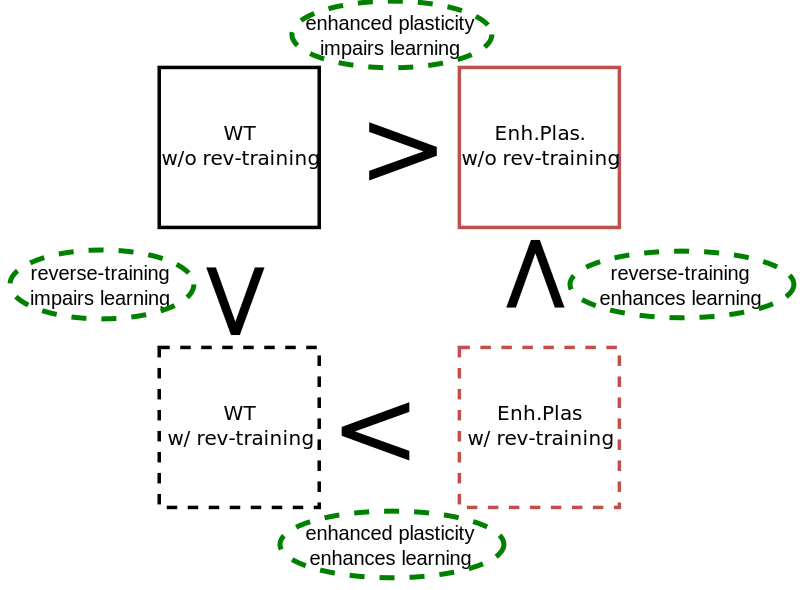
\includegraphics[width=0.55\linewidth]{comparisons_all.svg}}}
% \end{center}
% \note[item]{Restricted to gain inc for comparison}
%% \note[item]{Black: WT. Red: Enh.Plas}
% \note[item]{Solid: no pre. Dashed: with pre}
% \note[item]{Initial slope only}
%% \note[item]{Horz and vert comparisons: conceptual}
% \note[item]<2->{Enh.Plas. hurts w/o. Competition?}
% \note[item]<3->{Enh.Plas. helps w/. Expected}
% \note[item]<4->{now we can compare w/o,w/ rev}
% \note[item]<4->{rev helps Enh.Plas. as expected}
% \note[item]<5->{but rev hurts WT. Question}
% \note[item]<6>{Summarize: Enh.Plas. can impair/enhance. Rev can impair/enhance}
% \note[item]<6>{Diagonal comparisons: parameter fitting. Depend on size of mut vs.\ rev}
%% \note[item]{top and left most restrictive}
%% \note[item]{Pay attention to solid: black above red}
%% \note[item]{Pay attention to black: solid above dashed}
%% \note[item]{Concentrate on initial slope}
%
% \onslide<2->Questions:
%%
% \begin{itemize}
%   \item<2-> Can the depletion effect overcome enhanced intrinsic plasticity?
%%   \note[item]{in competition}
%   \item<5-> How can a little replenishment help, but too much hurt?
%%   \note[item]{first makes sense, but second?}
%%   \item Can we find a purely synaptic explanation of these results?
% \end{itemize}
%%
%%
%\end{frame}
%
%%-------------Slide--------------------------------------------------------
%
%\begin{frame}{Questions}
%%
% \begin{itemize}
%   \item Can the saturation effect overcome the enhanced plasticity?
%   \note[item]{in competition}
%   \item How can a little reverse bias help, but too much hurt?
%   \note[item]{first makes sense, but second?}
%   \item Can we find a purely synaptic explanation of these results?
%   \note[item]{This is a question about synaptic populations after all.}
% \end{itemize}
%%
%\end{frame}
%
%%-------------Section--------------------------------------------------------
%
%\section{Modelling approach}
%
%%-------------Slide--------------------------------------------------------
%
%\begin{frame}{Model of circuit}
%%
% %
% \begin{center}
%   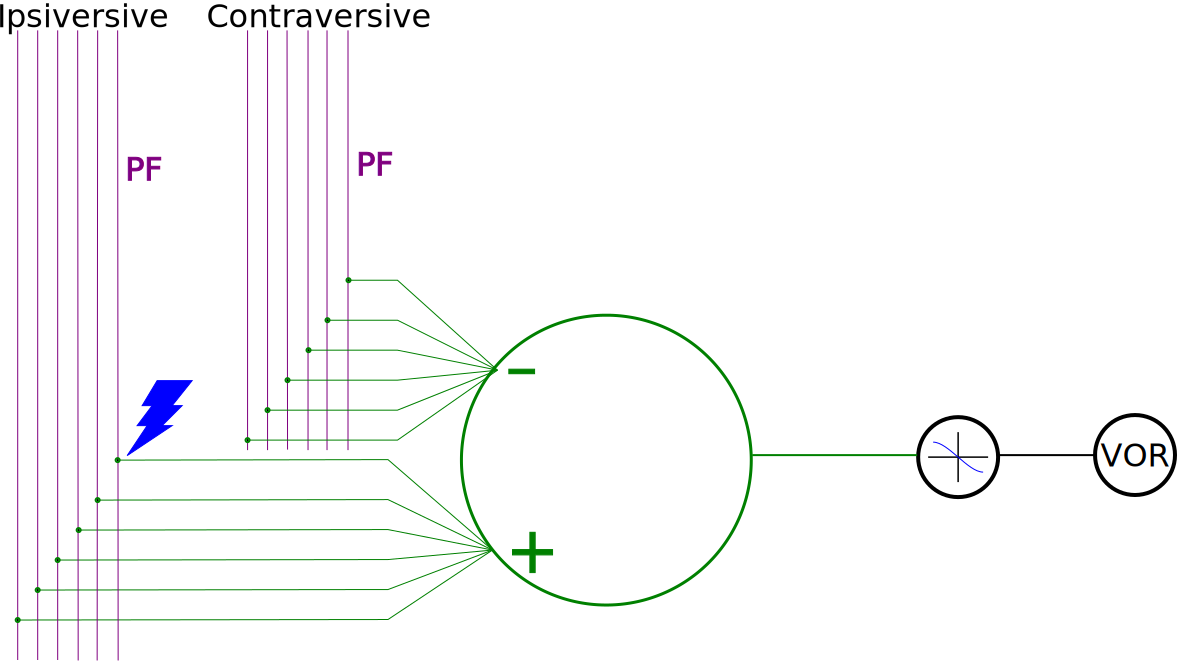
\includegraphics[width=0.9\linewidth]{VORmodel.svg}
% \end{center}
% %
% \note[item]{Contralateral baseline shift compensates for Our baseline shift}
% \note[item]{Gain increase due to LTD at lightning}
% \note[item]{Gain decease due to plasticity elsewhere, but also reverses LTD at lightning.}
% \note[item]{Nonlinearity here won't affect our questions, as long as it doesn't change}
% \note[item]{Nonlinearity before compensation could change things}
%%
%\end{frame}

%%-------------Slide--------------------------------------------------------
%
%\begin{frame}{Behaviour to synapses}
%%
%\begin{center}
% \alignmid{
\includegraphics[width=0.3\linewidth]{VORinc.svg}}
% \hspace{0.2\linewidth}
% \alignmid{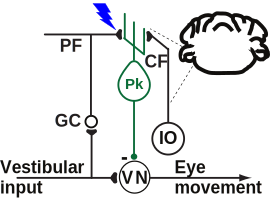
\includegraphics[width=0.4\linewidth]{VORcircuit.svg}}
% \note[item]{Focus on synapses. See if we can understand this behaviour.}
%\end{center}
%%
%\end{frame}
%%
%%-------------Slide--------------------------------------------------------
%
%\begin{frame}{Complex synapses}
%%
% \begin{center}
%  \aligntop{\includegraphics[width=4cm]{synapse.svg}}\hp
%  %
%  %
%  \hp\aligntop{\includegraphics[width=2cm]{pot.svg}}
%  \hp\aligntop{\includegraphics[width=2cm]{dep.svg}}
% \end{center}
%  %
%  \note[item]{Not just synaptic weight, internal dynamical system}
%  \note[item]{Important for memory: simple synapses -- terrible storage, rescued by complexity}
%  \note[item]{Multiple functional states w/ different weights}
%  \note[item]{Stochastic transitions between states}
%
%  \vp Assumptions:
%\begin{itemize}
%%  \item No spatial/temporal patterns in plasticity events.
%  \item Candidate plasticity events occur independently at each synapse,
%
%  \item Each synapse responds with the same state-dependent rules,
%      %
%%      \note[item]{pot/dep occur randomly}
%      %
%%  \item \rule{0mm}{0mm}\cancel{Synaptic identity} \lto\ synaptic distribution.
%  \item Keep track of distribution of synapses across states.
%      %
%      \note[item]{allows us to concentrate on synapse, not neuron/network}
%      \note[item]{This is a question about synaptic populations after all.}
%%  \item Potentiating/depressing plasticity events $\sim$ Poisson processes.% with rates $rf\potdep$, where $f\pot+f\dep=1$.
%%      %
%%      \note[item]{don't care if STDP...}
%%      %
%%  \item Potentiation and depression are described by Markov processes.% with transition probabilities $\M\potdep$.
%%      %
%\end{itemize}
%  \vp\citerr{Fusi2005cascade,Fusi2007multistate,Barrett2008discrete}
%%
%\end{frame}
%
%%-------------Slide--------------------------------------------------------
%
%\begin{frame}{Simplifying assumptions}
%%
%\begin{itemize}
%  \item No spatial/temporal correlations in plasticity events.
%      %
%      \note[item]{allows us to concentrate on synapse, not neuron/network}
%      %
%%  \item Which synapses eligible for plasticity chosen randomly.
%      %
%      \note[item]{No filing system}
%      %
%  \vp\item Potentiating/depressing plasticity events $\sim$ Poisson processes.% with rates $rf\potdep$, where $f\pot+f\dep=1$.
%      %
%      \note[item]{don't care if STDP...}
%%      %
%%      \note[item]{$r=$ total rate of plasticity events per synapse, $f\potdep=$ fraction of events that are potentiating/depressing.}
%      %
%  \vp\item Potentiation and depression are described by Markov processes.% with transition probabilities $\M\potdep$.
%%      %
%%      \note[item]{matrix elements: transition prob from $i\to j$, given pot/dep}
%%  \item Ideal observer: read weights directly.
%%      \note[item]{not electrical activity: don't model neurons/network}
%%      \note[item]{upper bound on electrical activity readout}
%%      %
%%  \item Synaptic weights can only take values $\pm1$.
%%      %
%%      \note[item]{looks like binary synapse from outside. Inside...}
%      %
%  \vp\citerr{Fusi2005cascade,Fusi2007multistate,Barrett2008discrete}
%\end{itemize}
%%
%\end{frame}
%

%-------------Slide--------------------------------------------------------

\begin{frame}{Synapses are complex}
%
 \parbox[t]{0.45\linewidth}{%
 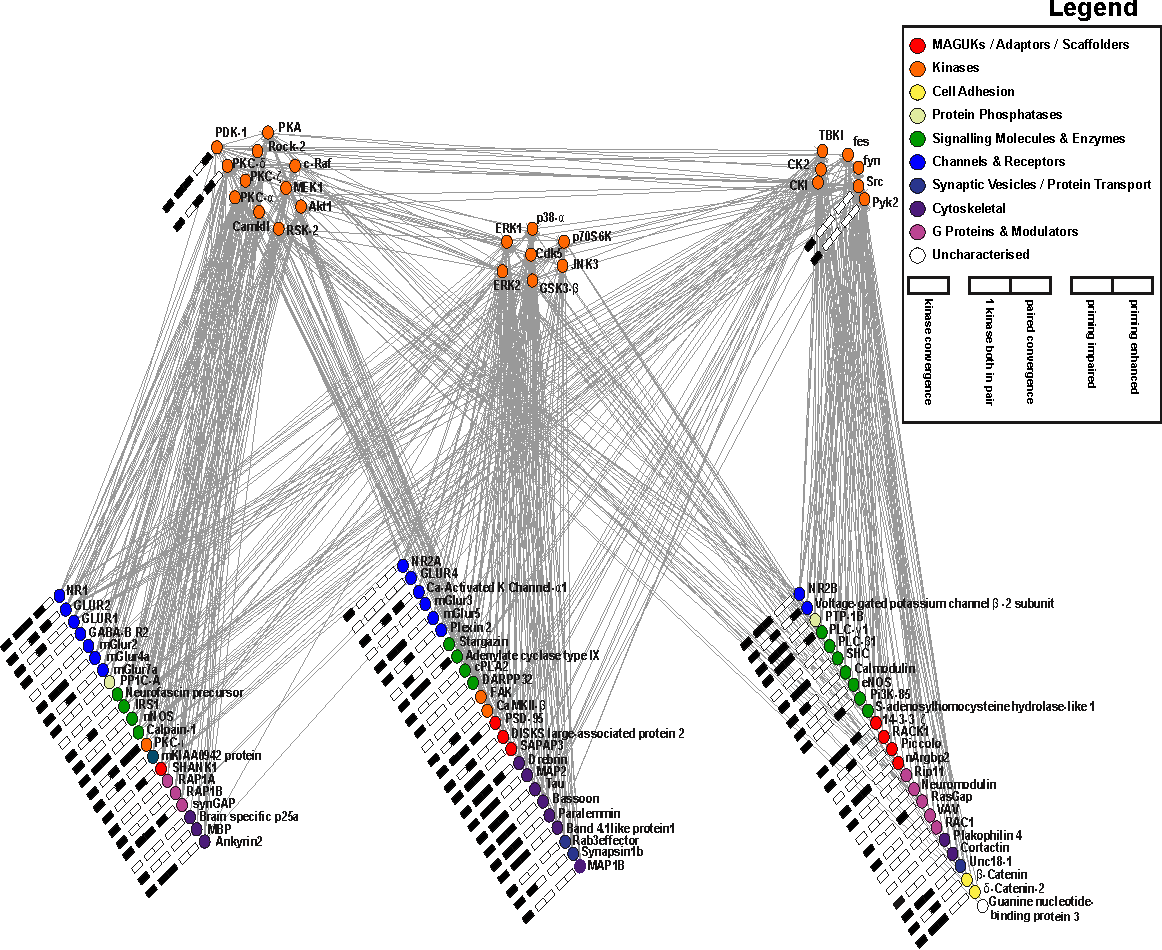
\includegraphics[height=0.8\linewidth]{2000102CobaFig4.pdf}

 \citerr{Coba2009phosphorylation}
 }
 \hspace{0.05\linewidth}
 \parbox[t]{0.45\linewidth}{%
 \hfill
 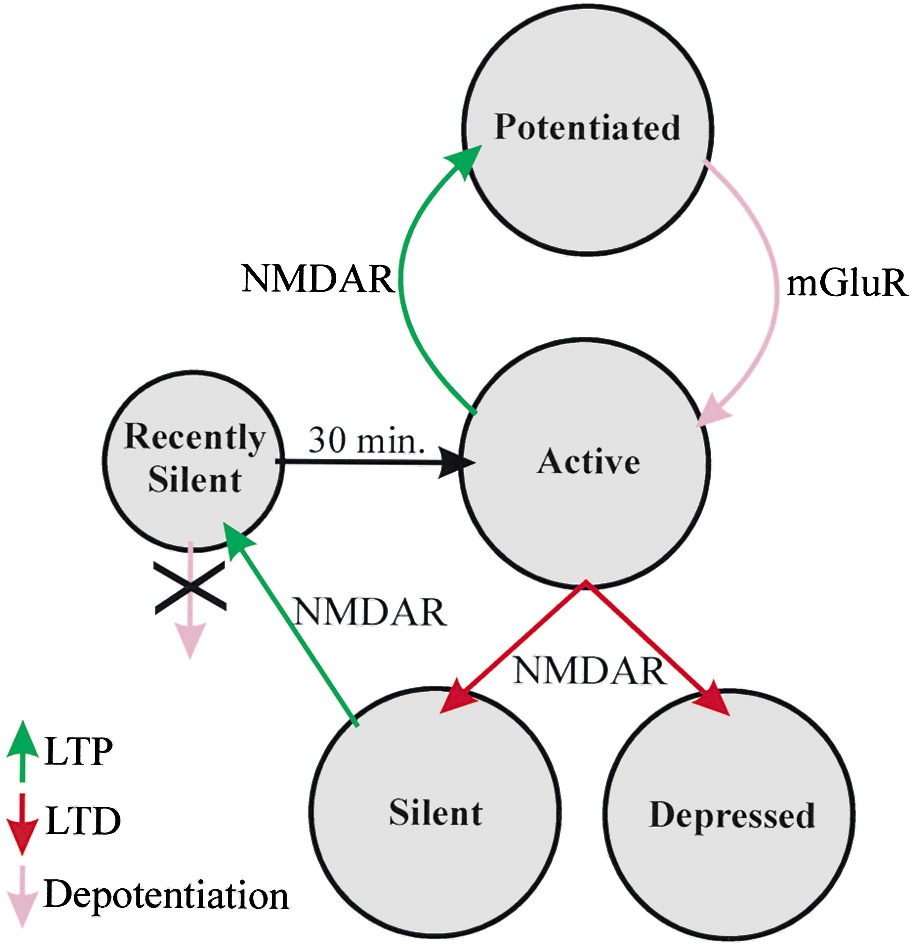
\includegraphics[height=0.8\linewidth]{MadisonMontgomery.jpg}

 \citerr{Montgomery2002765}
 }
%
\end{frame}

%-------------Slide--------------------------------------------------------

\begin{frame}{Models of complex synaptic dynamics}
%
%  There are $N$ identical synapses with $M$ internal functional states.
\parbox[c]{0.82\linewidth}{%
  \begin{itemize}
    \item Internal functional state of synapse \lto\ synaptic weight.
    \item Candidate plasticity events \lto\ transitions between states
  \end{itemize}
}\hfill
\alignmid{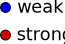
\includegraphics[width=0.13\linewidth]{state_key.svg}}
  %
  \vp
  \begin{center}
%  \begin{overlayarea}{0.7\linewidth}{0.3\linewidth}
%    \only<1>{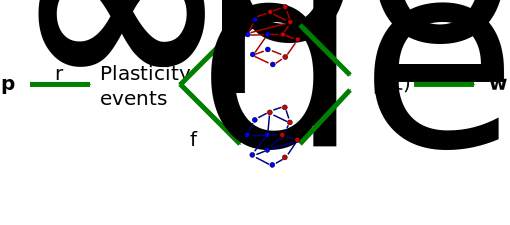
\includegraphics[width=0.99\linewidth]{synapse_model_1.svg}}%
%    \only<2>{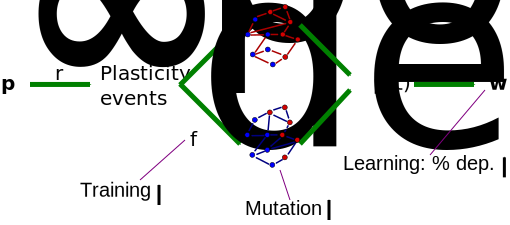
\includegraphics[width=0.99\linewidth]{synapse_model_2.svg}}
%  \end{overlayarea}
%    \aligntop{\movie[width=200px,height=92px,showcontrols=true,loop]{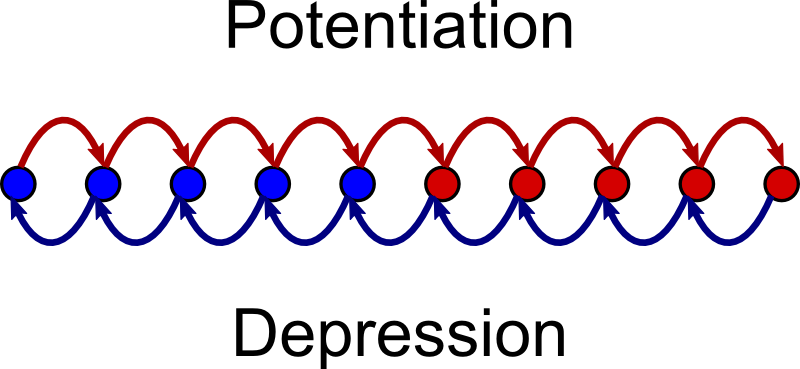
\includegraphics[width=200px,height=92px]{Vids/plast_00.png}}{plast.avi}}
    \only<1>{\aligntop{\includegraphics[width=0.5\linewidth]{Animation/serial.svg}}}%
    \only<2>{\aligntop{\includegraphics[width=0.5\linewidth]{Animation/serial_anim_01.svg}}}%
    \only<3>{\aligntop{\includegraphics[width=0.5\linewidth]{Animation/serial_anim_02.svg}}}%
    \only<4>{\aligntop{\includegraphics[width=0.5\linewidth]{Animation/serial_anim_03.svg}}}%
%    \only<5>{\aligntop{\includegraphics[width=0.5\linewidth]{Animation/serial_anim_04.svg}}}%
%    \only<6>{\aligntop{\includegraphics[width=0.5\linewidth]{Animation/serial_anim_05.svg}}}%
%    \only<7>{\aligntop{\includegraphics[width=0.5\linewidth]{Animation/serial_anim_06.svg}}}%
%    \only<8>{\aligntop{\includegraphics[width=0.5\linewidth]{Animation/serial_anim_07.svg}}}%
%    \only<9>{\aligntop{\includegraphics[width=0.5\linewidth]{Animation/serial_anim_08.svg}}}%
%    \only<10>{\aligntop{\includegraphics[width=0.5\linewidth]{Animation/serial_anim_09.svg}}}%
%    \only<11>{\aligntop{\includegraphics[width=0.5\linewidth]{Animation/serial_anim_10.svg}}}%
%    \only<12>{\aligntop{\includegraphics[width=0.5\linewidth]{Animation/serial_anim_11.svg}}}%
%    \only<13>{\aligntop{\includegraphics[width=0.5\linewidth]{Animation/serial_anim_12.svg}}}%
%    \only<14>{\aligntop{\includegraphics[width=0.5\linewidth]{Animation/serial_anim_13.svg}}}%
%    \only<15>{\aligntop{\includegraphics[width=0.5\linewidth]{Animation/serial.svg}}}%
    \only<5>{\aligntop{\includegraphics[width=0.5\linewidth]{Animation/serial_anim_06.svg}}}%
    \only<6>{\aligntop{\includegraphics[width=0.5\linewidth]{Animation/serial_anim_07.svg}}}%
    \only<7>{\aligntop{\includegraphics[width=0.5\linewidth]{Animation/serial_anim_08.svg}}}%
    \only<8>{\aligntop{\includegraphics[width=0.5\linewidth]{Animation/serial_anim_09.svg}}}%
    \only<9>{\aligntop{\includegraphics[width=0.5\linewidth]{Animation/serial_anim_10.svg}}}%
    \only<10>{\aligntop{\includegraphics[width=0.5\linewidth]{Animation/serial_anim_11.svg}}}%
    \only<11>{\aligntop{\includegraphics[width=0.5\linewidth]{Animation/serial_anim_12.svg}}}%
    \only<12>{\aligntop{\includegraphics[width=0.5\linewidth]{Animation/serial_anim_13.svg}}}%
    \only<13>{\aligntop{\includegraphics[width=0.5\linewidth]{Animation/serial.svg}}}%
    %
    \hspace{0.05\linewidth}\parbox[t]{0.45\linewidth}{\raggedright
    \visible<13>{
    Mutation: transition probabilities \\ \vp
    Training: rates of pot/dep events \\ \vp
    Learning: synaptic weight}}
  \end{center}

%  \onslide<2>{\hfill
%  \parbox[t]{0.3\linewidth}{PF+\cancel{CF} \lto\ LTP, \\
%              PF+CF \lto\ LTD.}
%  \parbox[t]{0.27\linewidth}{Lower threshold\\ for LTD}
%  \parbox[t]{0.27\linewidth}{VOR gain increase}}

  \vp
  \footnotesize\citerr{Fusi2005cascade,Fusi2007multistate,Barrett2008discrete}\\\citerr{Smith2006savings,Lahiri2013synapse}

  %
  \note[item]{complex synapse: not just synaptic weight. dynamical system}
  \note[item]{important for memory with bounded synapses}
  \note[item]{nodes \lto\ states}
  \note[item]{color \lto\ sttrength}
  \note[item]{arrows \lto\ plasticity}
%  \note[item]{stoch process has steady state distribution.}
%  \note[item]{Prior activity puts it in this state. row vec.}
  \note[item]{plasticity events at rate r. indep at each synapse.}
  \note[item]{fraction pot/dep}
  \note[item]{Readout: synaptic weight vec when in each state.}
    \note[item]{Mutation: lower threshold \lto\ increase transition probs}
    \note[item]{Training: Changes statistics of LTP/LTD. Only parameters we have. Don't care about $r$.}
    \note[item]{Learning: Only output we have. Don't keep track of synaptic identity.}
%    \note<2>[item]{Same PF+CF input \lto\ same $r,f\pot,f\dep$ in each case.}
%    \note<2>[item]{Input to Pk, some linear combination of $\w$'s. }
% At $t=0$, the memory is created by $\M\potdep$ with probability $f\potdep$.
% \note[item]{for this one, we keep track of pot/dep, look for inc/dec of $\w$}
%
% \vp Forgetting caused by subsequent memories, evolving as
%
%  \begin{equation*}
%  \begin{aligned}
%    \diff{\pr(t)}{t} &= r\pr(t)\frg,
%    &\qquad
%    \frg &= f\pot\M\pot+f\dep\M\dep-\I,\\&&
%    \eq\frg &=0.
%  \end{aligned}
%  \end{equation*}
%%
%  \note[item]{Memory at $t=0$, keep track of pot/dep}
%  \note[item]{subsequent: average over pot/dep}
% \note[item]{$\frg$ is forgetting matrix, $\I=$identity, don't keep track of pot/dep}
% Eventually, this will settle into the equilibrium distribution:
% %
% %
% \note[item]{In equilibrium prior to memory creation}
%
\end{frame}

%-------------Slide--------------------------------------------------------

\begin{frame}{Questions}
%
 Depletion effect competes with enhanced intrinsic plasticity.
 
 \vp\alert{Question 1:}  When is the depletion effect stronger?
  
 \vp\vp\vp Reverse training impairs learning in wild-type.  
 
 \vp\alert{Question 2:} How can replenishment \emph{ever} impair learning?
%
\end{frame}

%%-------------Slide--------------------------------------------------------
%
%\begin{frame}{Modelling VOR learning}
%%
%\begin{tabular}{>{\bfseries}ll>{\impl}l}
%    Mutation: &
%    Changes mechanism of LTD  &
%    change $\M\dep$.
%    \note[item]{lower threshold \lto\ increase off-diagonal elements.}
% \\[1cm]
%    Training: &
%    Changes statistics of LTP/LTD  &
%    change $r,f\pot,f\dep$.
%    \note[item]{Only parameters we have. Don't care about $r$.}
%    \note[item]{Same PF+CF input \lto\ same $r,f\pot,f\dep$ in each case.}
% \\[1cm]
%    Learning: &
%    Change in VOR gain &
%    fn.\ of decrease in $\av{\w}$.
%    \note[item]{Only output we have. Don't keep track of synaptic identity.}
%    \note[item]{Input to Pk, some linear combination of $\w$'s. }
%\end{tabular}
%%
%\end{frame}
%
%%-------------Section--------------------------------------------------------
%
%\section{Modelling results}
%
%%-------------Slide--------------------------------------------------------
%
%\begin{frame}{Binary synapse}
%%
% %
% \begin{center}
%   \includegraphics[width=0.15\linewidth]{binary.svg} \\[1cm]
%   \aligntop{\includegraphics[width=0.35\linewidth]{binary_learnS.eps}}
%   \hspace{2cm}
%   \aligntop{\includegraphics[width=0.35\linewidth]{comparisons_binary.svg}}
% \end{center}
% %
% \note[item]{Compare solid curves}
% \note[item]{Compare black curves}
% \note[item]{understand why next slide}
%%
%\end{frame}
%
%%-------------Slide--------------------------------------------------------
%
%\begin{frame}{Binary synapse}
%%
% %
%\adjustbox{valign=m}{\parbox[t]{0.4\linewidth}{
%  \begin{raggedleft}
%  Learning rate: \phantom{rate of events} \\
%  \hp\hp\parbox{0.75\linewidth}{%
%  $\sim$ rate of events\\
%  $\times$ prob.\ of transition\\
%  $\times$ prob.\ ready for $\Delta w$\\
%  $\times$ (-$\Delta w$)}
%  \end{raggedleft}
%}}
%% \begin{center}
%\alignmid{\parbox[t]{0.5\linewidth}{
% \begin{tabular}{ccc}
%   \alignmid{\includegraphics[height=0.5\linewidth]{binary_bar_wt_wo.svg}}
%   & \alignmid{\includegraphics[height=0.12\linewidth]{left_bad.svg}} &
%   \alignmid{\includegraphics[height=0.5\linewidth]{binary_bar_ko_wo.svg}}
%   \\[1.5cm] \alignmid{\includegraphics[height=0.12\linewidth]{up_bad.svg}}
%   && \alignmid{\includegraphics[height=0.12\linewidth]{up_good.svg}}\\[0.5cm]
%   \alignmid{\includegraphics[height=0.5\linewidth]{binary_bar_wt_w.svg}}
%   & \alignmid{\includegraphics[height=0.12\linewidth]{left_good.svg}} &
%   \alignmid{\includegraphics[height=0.5\linewidth]{binary_bar_ko_w.svg}}
% \end{tabular}
%}}
%% \end{center}
% %
% \note[item]{WT: start with everything equal -- just for illustration, not essential}
% \note[item]{WT: during training, increase $f\dep$ (green arrow) $\to$ weakening.}
% \note[item]{KO: inc $q\pot\to$ bias}
% \note[item]{KO: competition between inc prob trans \& dec prob ready}
% \note[item]{KO: first one wins. see why after next model}
% \note[item]{pre: reduces/reverses bias. always helps.}
%%
%\end{frame}
%
%%-------------Slide--------------------------------------------------------
%
%\begin{frame}{Serial synapse}
%%
% %
% \begin{center}
%   \includegraphics[width=0.5\linewidth]{serial.svg}\\
%   \citerr{Leibold2008serial} \\[1cm]
% \note[item]{Still looks binary from outside. Hidden states (not essential).}
% \note[item]{Only see $\Delta w$ at boundary.}
%   \aligntop{\includegraphics[width=0.35\linewidth]{serial_learnS.eps}}
%   \hspace{2cm}
%   \aligntop{\includegraphics[width=0.35\linewidth]{comparisons_serial.svg}}
% \end{center}
% %
%
% \note[item]{understand why next slide}
%%
%\end{frame}
%
%%-------------Slide--------------------------------------------------------
%
%\begin{frame}{Serial synapse}
%%
%   \citerr{Leibold2008serial} \\
% %
% \begin{center}
% \begin{tabular}{ccc}
%   \alignmid{\includegraphics[height=0.19\linewidth]{serial_bar_wt_wo.svg}}
%   & \alignmid{\includegraphics[height=0.05\linewidth]{right_good.svg}} &
%   \alignmid{\includegraphics[height=0.19\linewidth]{serial_bar_ko_wo.svg}}
%   \\[1.5cm] \alignmid{\includegraphics[height=0.05\linewidth]{down_good.svg}}
%   && \alignmid{\includegraphics[height=0.05\linewidth]{up_good.svg}}\\[0.5cm]
%   \alignmid{\includegraphics[height=0.19\linewidth]{serial_bar_wt_w.svg}}
%   & \alignmid{\includegraphics[height=0.05\linewidth]{left_good.svg}} &
%   \alignmid{\includegraphics[height=0.19\linewidth]{serial_bar_ko_w.svg}}
% \end{tabular}
% \end{center}
% %
% \note[item]{Now only get signal from crossing boundary}
% \note[item]{KO: inc $q\pot\to$ bias, now exponential}
% \note[item]{KO: prob ready wins over prob trans, now exponential}
% \note[item]{pre: reduces/reverses bias.}
% \note[item]{pre: little reverse bias repopulates bndry, helps.}
% \note[item]{pre: too much reverse bias moves away from bndry, hurts.}
% \note[item]{maths next slide}
%%
%\end{frame}
%
%%-------------Slide--------------------------------------------------------
%
%\begin{frame}{Mathematical explanation}
%%
% %
% \begin{center}
%   \includegraphics[width=0.4\linewidth]{serial_label.svg}
% \end{center}
% %
% \vp Serial synapse: $\eq_i \sim \CN \prn{\frac{q\pot}{q\dep}}^i$.
%
% \vp Learning rate $\sim \eq_{M/2}\prn{\frac{q\dep}{q\pot}} = \CN \prn{\frac{q\pot}{q\dep}}^{\frac{M}{2}-1}$.
% \note[item]{Detailed balance. Exponential decay.}
%
% \vp For $M>2$: larger $q\dep \implies$ slower learning.
% \note[item]{for large enough $M,q\pot$, overcome $\CN$}
%
% \vp For $M=2$: larger $q\dep \implies$ larger $\CN \implies$ faster learning.
% \note[item]{Other factor in $\eq$ smaller $\implies \CN$ larger.}
%%
%\end{frame}
%
%%-------------Slide--------------------------------------------------------
%
%\begin{frame}{Model results}
%%
% \begin{center}
% \begin{tabular}{c@{\hspace{0.1\linewidth}}c}
%   Binary model & Serial Model \\[0.5cm]
%   \alignmid{\includegraphics[height=0.07\linewidth]{binary.svg}} &
%   \alignmid{\includegraphics[height=0.07\linewidth]{serial.svg}}\\[1cm]
%   \aligntop{\includegraphics[height=0.35\linewidth]{binary_learnS.svg}} &
%   \aligntop{\includegraphics[height=0.35\linewidth]{serial_learnS.svg}}
% \end{tabular}
% \end{center}
% \note[item]{Binary fails -- mathematical prrof for any params}
% \note[item]{Enh.Plas: faster depression wins over bias}
% \note[item]{pre: reduces/reverses bias. always helps.}
% \note[item]{Serial: still only two weights. Works.}
% \note[item]{Understand by looking at distributions before training}
% \citerr{Leibold2008serial}
%%
%\end{frame}
%
%-------------Slide--------------------------------------------------------

\begin{frame}{Simple synapses cannot explain the data}
%
 \begin{center}
 \begin{tabular}{c@{\hspace{0.1\linewidth}}c}
   \only<1>{\aligntop{\includegraphics[height=0.15\linewidth]{multistate.svg}}}%
   \only<2-6>{\aligntop{\includegraphics[height=0.15\linewidth]{binary.svg}}}%
   &
   \visible<1-3,5,6>{\aligntop{\includegraphics[height=0.19\linewidth]{VORinc.svg}}}\\[2cm]
   \only<1>{\aligntop{\includegraphics[width=0.35\linewidth]{blank_learnS.svg}}}%
   \only<2>{\aligntop{\includegraphics[width=0.35\linewidth]{binary_learnS.svg}}}%
   \only<3>{\aligntop{\includegraphics[width=0.35\linewidth]{binary_learnS_top.svg}}}%
   \only<4>{\aligntop{\includegraphics[width=0.35\linewidth]{binary_bar_ko_wo_s.svg}}}%
   \only<5>{\aligntop{\includegraphics[width=0.35\linewidth]{binary_learnS_left.svg}}}%
   \only<6>{\aligntop{\includegraphics[width=0.35\linewidth]{binary_bar_wt_w_s.svg}}}%
   &
   \only<1-2>{\aligntop{\includegraphics[width=0.35\linewidth]{data_shifted_nl.svg}}}%
   \only<3>{\aligntop{\includegraphics[width=0.35\linewidth]{data_shifted_top_nl.svg}}}%
   \only<4>{\parbox[t]{0.35\linewidth}{\centering \vp depletion effect\\ $<$ \\ enhanced plasticity \\
   \vp $\implies$  enhanced learning}}%
   \only<5>{\aligntop{\includegraphics[width=0.35\linewidth]{data_shifted_left_nl.svg}}}%
   \only<6>{\parbox[t]{0.35\linewidth}{\centering \vp reverse training\\ $\implies$ \\ replenishment \\
    $\implies$ \\ enhanced learning}}%
 \end{tabular}
 \end{center}
 \note[item]{Binary fails -- mathematical proof for any params}
 \note[item]{Enh.Plas: faster depression wins over bias}
 \note[item]{pre: reduces/reverses bias. always helps.}
%
\end{frame}

%-------------Slide--------------------------------------------------------

\begin{frame}{Complex metaplastic synapses can explain the data}
%
 \begin{center}
 \begin{tabular}{c@{\hspace{0.1\linewidth}}c}
   \aligntop{\includegraphics[height=0.15\linewidth]{serial.svg}} &
   \visible<1,2,4>{\aligntop{\includegraphics[height=0.19\linewidth]{VORinc.svg}}}\\[2cm]
   \only<1>{\aligntop{\includegraphics[height=0.35\linewidth]{serial_fit_learnS.svg}}}%
   \only<2>{\aligntop{\includegraphics[height=0.35\linewidth]{serial_fit_learnS_top.svg}}}%
   \only<3>{\aligntop{\includegraphics[height=0.35\linewidth]{serial_bar_ko_wo_s.svg}}}%
   \only<4>{\aligntop{\includegraphics[height=0.35\linewidth]{serial_fit_learnS_left.svg}}}%
%   \only<3>{\aligntop{\includegraphics[height=0.35\linewidth]{serial_bar_ko_w_s.svg}}}%
   \only<5>{\aligntop{\includegraphics[height=0.35\linewidth]{serial_bar_wt_w_s.svg}}}%
   &
   \only<1>{\aligntop{\includegraphics[height=0.35\linewidth]{data_shifted_nl.svg}}}%
   \only<2>{\aligntop{\includegraphics[height=0.35\linewidth]{data_shifted_top_nl.svg}}}%
   \only<3>{\parbox[t]{0.35\linewidth}{\centering \vp amplified depletion\\ $>$ \\ enhanced plasticity \\
   \vp $\implies$  impaired learning}}%
%   \only<3>{\aligntop{\includegraphics[height=0.35\linewidth]{data_shifted_right_nl.svg}}}%
   \only<4>{\aligntop{\includegraphics[height=0.35\linewidth]{data_shifted_left_nl.svg}}}%
   \only<5>{\parbox[t]{0.35\linewidth}{\centering \vp reverse training\\ $+$ \\ ``stubborn'' metaplasticity \\
   \vp $\implies$  impaired learning}}%
 \end{tabular}
 \end{center}
%  \visible<3>{\alert{Key:} ``Stubborn'' metaplasticity}\\
 \citerr{Leibold2008serial,Ben-DayanRubin2007sparse}

 \note[item]{Serial: still only two weights. Works.}
 \note[item]{Understand by looking at distributions before training}
%
\end{frame}

%%-------------Slide--------------------------------------------------------
%
%\begin{frame}{Complex synapses are required to explain behaviour}
%%
% \begin{center}
% \begin{tabular}{c@{\hspace{0.05\linewidth}}c@{\hspace{0.05\linewidth}}c}
%   \aligntop{\includegraphics[height=0.12\linewidth]{binary.svg}} &
%   \aligntop{\includegraphics[height=0.12\linewidth]{serial.svg}} &
%   \aligntop{\includegraphics[height=0.2\linewidth]{VORinc.svg}}\\[2.5cm]
%   \aligntop{\includegraphics[height=0.27\linewidth]{binary_learnS.svg}} &
%   \aligntop{\includegraphics[height=0.27\linewidth]{serial_fit_learnS.svg}} &
%   \aligntop{\includegraphics[height=0.27\linewidth]{data_shifted.svg}}
% \end{tabular}
% \end{center}
% \note[item]{Binary fails -- mathematical proof for any params}
% \note[item]{Enh.Plas: faster depression wins over bias}
% \note[item]{pre: reduces/reverses bias. always helps.}
% \note[item]{Serial: still only two weights. Works.}
% \note[item]{Understand by looking at distributions before training}
% \citerr{Leibold2008serial,Ben-DayanRubin2007sparse}
%%
%\end{frame}
%
%-------------Slide--------------------------------------------------------

\begin{frame}{Enhanced plasticity can enhance or impair learning}
%
 %
 \begin{center}
 \begin{tabular}{c@{\hspace{0.1\linewidth}}c}
   {\includegraphics[height=0.2\linewidth]{binary_bar_ko_wo_s.svg}}&
   {\includegraphics[height=0.2\linewidth]{serial_bar_ko_wo_s.svg}}\\[1cm]
   Intrinsic plasticity  & Depletion dominates \\
   dominates depletion & intrinsic plasticity\\
   $\downarrow$ & $\downarrow$ \\
   enhanced plasticity & enhanced plasticity \\
   enhances learning & impairs learning
 \end{tabular}
 \end{center}
 \note[item]{Binary: enhanced plasticity \lto\ bias}
 \note[item]{Not enough to overcome faster depression}
 \note[item]{Serial: Only get signal from boundary}
 \note[item]{Exponential decay depopulates boundary, enhances effect of bias}
 %

 \vp\alert{Key feature 1:} Synaptic complexity that amplifies depletion effect.
 \note[item]{borne out by other models}
%
\end{frame}

%-------------Slide--------------------------------------------------------

\begin{frame}{Reverse-training can impair or enhance learning}
%
 %
 \begin{center}
 \begin{tabular}{c@{\hspace{0.1\linewidth}}c}
   {\includegraphics[height=0.2\linewidth]{binary_bar_wt_w_s.svg}}&
   {\includegraphics[height=0.2\linewidth]{serial_bar_wt_w_s.svg}}
%   &
%   {\includegraphics[height=0.2\linewidth]{serial_bar_ko_w_s.svg}}
   \\[1cm]
   reverse-training &
   reverse-training \\
   repopulates boundary
   &
   depopulates boundary 
%   &
%   repopulates boundary
   \\
   $\downarrow$ & $\downarrow$ \\
   enhanced learning
   &
   impaired learning 
%   &
%   enhanced learning
 \end{tabular}
 \end{center}
 \note[item]{rev-training: little repopulates boundary}
 \note[item]{Too much pushes to other side, depopulates boundary}
 \note[item]{this effect is absent in any simple synapse}

 \vp\alert{Key feature 2:} ``Stubborn'' metaplasticity.
 \note[item]{repeated potentiation makes subsequent depression harder}
 \note[item]{borne out by other models}
 %
%
\end{frame}

%-------------Slide--------------------------------------------------------

\begin{frame}{Essential features}
%
 %
 \begin{center}
   \includegraphics[width=0.4\linewidth]{serial_s.svg}
 \end{center}
 %
 \vp The success of the serial model relies on two features:
 \begin{itemize}
   \item Complexity - needed to amplify the effect of depletion,
   \note[item]{due to exponential decay}
   \item Metaplasticity -- repeated potentiation impairs subsequent depression.
   \note[item]{push away from boundary where signal generated}
 \end{itemize}
 \note[item]{borne out by other models that fail/succeed}

 %\visible<2>{
 \begin{center}
 \begin{tabular}{c@{\hp\hp}c}
    Fail:&
    Succeed:\\[0.3cm]
    \aligntop{\includegraphics[width=0.3\linewidth]{pooled_s.svg}}&
    \aligntop{\includegraphics[width=0.3\linewidth]{cascade_s.svg}}\\[1.5cm]
    \aligntop{\includegraphics[width=0.3\linewidth]{multistate_s.svg}}&
    \aligntop{\includegraphics[width=0.3\linewidth]{multistate_nonuni_s.svg}}
 \end{tabular}
 \end{center}
 \citerr{amit1994learning,Fusi2005cascade}
 %}
%
\end{frame}

%%%-------------Slide--------------------------------------------------------
%
%\begin{frame}{Other models that fail}
%%
% \begin{tabular}{ll}
%   % & for next tab, \\ for new line...
%    \aligntop{\includegraphics[width=0.4\linewidth]{multistate.svg}}\hspace{1.5cm} &
%    \aligntop{\includegraphics[width=0.28\linewidth]{multistate_learnS.eps}}
%    \note[item]{MS: linear weights, unlike serial.}
%    \note[item]{like bunch of binary synapses in series.}
%    \note[item]{solid curves: fails early on , but catches up quickly}
%    \note[item]{black curves: fails badly}
%    \note[item]{No real enhancement of saturation, no metaplasticity.}
%    \note[item]{All transitions contribute: pushing to end has little effect.}
%    \\[2cm]
%    \aligntop{\includegraphics[width=0.4\linewidth]{pooled.svg}} &
%    \aligntop{\includegraphics[width=0.28\linewidth]{pooled_scarce_learnS.eps}}
%    \note[item]{Pooled: resource depleted by pot/dep. replenished by reverse.}
%    \note[item]{solid curves succeed: enhanced saturation}
%    \note[item]{black curves fail: opposite metaplasticity, pot makes dep easier}
% \end{tabular}
%
% \citerr{amit1994learning}
%%
%\end{frame}
%
%%-------------Slide--------------------------------------------------------
%
%\begin{frame}{Other models that work}
%%
% \begin{tabular}{ll}
%   % & for next tab, \\ for new line...
%    \aligntop{\includegraphics[width=0.4\linewidth]{multistate_nonuni.svg}}\hspace{1.5cm} &
%    \aligntop{\includegraphics[width=0.28\linewidth]{nonuni_learnS.eps}} \\[2cm]
%    \aligntop{\includegraphics[width=0.4\linewidth]{cascade.svg}} &
%    \aligntop{\includegraphics[width=0.28\linewidth]{cascade_long_learnS.eps}}
% \end{tabular}
% \note[item]{Both models, trans probs decay exponentially from centre.}
% \note[item]{Nonuni: linear weights. Cascade: binary weights.}
% \note[item]{Enhanced saturation and metaplasticity}
% \note[item]{Pushing to end makes pot and dep harder}
% \note[item]{Note: hidden states not necessary}
%
% \citerr{Fusi2005cascade}
%%
%\end{frame}
%
%-------------Slide--------------------------------------------------------

\begin{frame}{Conclusions}
%
 \begin{itemize}
%   \item The saturation effect can overcome faster depression, if it is enhanced.
%   \alert{Requires complexity}
%   \note[item]{\eg exponential deacy, resource depletion,\ldots}
%   \item A little reverse bias can help, but too much hurts, if repeated potentiation makes depression harder.
%   \alert{Requires metaplasticity}
%   \note[item]{\eg moving away from weight boundary, or weaker transitions.}
   \item Diverse behavioural patterns:\\
   \alert{Enhanced plasticity \lto\ enhance/impair} learning (prior experience).\\
   \alert{Reverse-training \lto\ enhance/impair} learning (plasticity rates).

   \item \alert{enhanced LTD} vs.\ \alert{depletion} \lto\ learning outcome.
    \hfill{\alignmid{\includegraphics[width=0.1\linewidth]{pinky_by_lonewolf16.jpg}}} {\alignmid{\includegraphics[width=0.07\linewidth]{the_brain_by_lonewolf16.jpg}}}



   \item Predictions for synaptic physiology:\\
   \alert{Synaptic complexity:} necessary to amplify depletion.\\
   \alert{Synaptic stubbornness:} repeated potentiation impairs future depression.

   \vp\item  We used behaviour to constrain the dynamics of synaptic plasticity
\end{itemize}
%
\end{frame}


%%-------------Slide--------------------------------------------------------
%
%\begin{frame}{Tradeoff: learning vs.\ remembering}
%%
% What about memory?
% \begin{itemize}
%   \vp\item Simple synapses have poor memory storage capacity. \\
%   Synaptic complexity is needed for rescue.\\
%   \citerr{amit1992constraints,amit1994learning}
%
%   \vp\item Trade-off between learning and remembering:\\
%   Too rigid \lto\ difficult to learn new memories.\\
%   Too plastic \lto\ new memories quickly overwrite old.
%
%   \vp\item Exploring the \emph{entire} space of complex synaptic models \\
%   \lto\ upper bounds on their storage ability \\
%   \& the models that saturate them.
% \end{itemize}
%
% \rref{Lahiri and Ganguli (submitted)}
%%
%\end{frame}
%
%%-------------Slide--------------------------------------------------------
%
%\begin{frame}{The frontiers of complex synaptic memory}
%%
% We have $N$ synapses with $M$ internal states each.
%
% \vp We study the decay of one memory over time due to corruption by subsequent memories.
%
% \vp We prove that, no matter what the structure, no synaptic model can have:\\
% \begin{itemize}
%   \item initial fidelity (SNR) greater than $\sqrt{N}$.
%   \item memory lifetime greater than $\sim\sqrt{N}M$.
%   \item fidelity decay slower than $\sim\sqrt{N}M/t$.
% \end{itemize}
%
% \vp At late times, fidelity is maximised by a model with a simple chain structure.
%%
%\end{frame}
%
%-------------Slide--------------------------------------------------------

\begin{frame}{Acknowledgements}
%
 \begin{tabular}{lll}
   \textbf{Surya Ganguli} & \textbf{Jennifer Raymond} & \textbf{Carla Shatz} \\
   Madhu Advani & Barbara Nguyen-Vu & Han-Mi Lee \\
   Peiran Gao & Grace Zhao & \\
   Niru Maheswaranathan & Aparna Suvrathan \\
   Ben Poole \\
   Jascha Sohl-Dickstein \\
   Kiah Hardcastle \\
   Jay Sarkar
 \end{tabular}

 \vp\textbf{Funding}: Swartz Foundation, Stanford Bio-X Genentech fellowship.

% \vp\textbf{Travel grant}: Gatsby Charitable Foundation,
%                           Qualcomm Incorporated,
%                           Brain Corporation,
%                           Evolved Machines.
%    \stoppagecounthere
%
\end{frame}

%-------------Slide--------------------------------------------------------
\appendix
%-------------Slide--------------------------------------------------------

\begin{frame}{Model of circuit}
%
 %
 \begin{center}
   \includegraphics[width=0.9\linewidth]{VORmodel.svg}
 \end{center}
 %
 \note[item]{Contralateral baseline shift compensates for Our baseline shift}
 \note[item]{Gain increase due to LTD at lightning}
 \note[item]{Gain decease due to plasticity elsewhere, but also reverses LTD at lightning.}
 \note[item]{Nonlinearity here won't affect our questions, as long as it doesn't change}
 \note[item]{Nonlinearity before compensation could change things}
%
\end{frame}
%%-------------Slide--------------------------------------------------------

\begin{frame}{Other models that fail}
%
 \begin{tabular}{ll}
   % & for next tab, \\ for new line...
    \aligntop{\includegraphics[width=0.4\linewidth]{multistate.svg}}\hspace{1.5cm} &
    \aligntop{\includegraphics[width=0.28\linewidth]{multistate_learnS.eps}}
    \note[item]{MS: linear weights, unlike serial.}
    \note[item]{like bunch of binary synapses in series.}
    \note[item]{solid curves: fails early on , but catches up quickly}
    \note[item]{black curves: fails badly}
    \note[item]{No real enhancement of saturation, no metaplasticity.}
    \note[item]{All transitions contribute: pushing to end has little effect.}
    \\[2cm]
    \aligntop{\includegraphics[width=0.4\linewidth]{pooled.svg}} &
    \aligntop{\includegraphics[width=0.28\linewidth]{pooled_scarce_learnS.eps}}
    \note[item]{Pooled: resource depleted by pot/dep. replenished by reverse.}
    \note[item]{solid curves succeed: enhanced saturation}
    \note[item]{black curves fail: opposite metaplasticity, pot makes dep easier}
 \end{tabular}

 \citerr{amit1994learning}
%
\end{frame}

%-------------Slide--------------------------------------------------------

\begin{frame}{Other models that work}
%
 \begin{tabular}{ll}
   % & for next tab, \\ for new line...
    \aligntop{\includegraphics[width=0.4\linewidth]{multistate_nonuni.svg}}\hspace{1.5cm} &
    \aligntop{\includegraphics[width=0.28\linewidth]{nonuni_fit_learnS.eps}} \\[2cm]
    \aligntop{\includegraphics[width=0.4\linewidth]{cascade.svg}} &
    \aligntop{\includegraphics[width=0.28\linewidth]{cascade_fit_learnS.eps}}
 \end{tabular}
 \note[item]{Both models, trans probs decay exponentially from centre.}
 \note[item]{Nonuni: linear weights. Cascade: binary weights.}
 \note[item]{Enhanced saturation and metaplasticity}
 \note[item]{Pushing to end makes pot and dep harder}
 \note[item]{Note: hidden states not necessary}

 \citerr{Fusi2005cascade}
%
\end{frame}

%-------------Slide--------------------------------------------------------

\begin{frame}{Mathematical explanation}
%
 %
 \begin{center}
   \includegraphics[width=0.4\linewidth]{serial_label.svg}
 \end{center}
 %
 \vp Serial synapse: $\eq_i \sim \CN \prn{\frac{q\pot}{q\dep}}^i$.

 \vp Learning rate $\sim \eq_{M/2}\prn{\frac{q\dep}{q\pot}} = \CN \prn{\frac{q\pot}{q\dep}}^{\frac{M}{2}-1}$.
 \note[item]{Detailed balance. Exponential decay.}

 \vp For $M>2$: larger $q\dep \implies$ slower learning.
 \note[item]{for large enough $M,q\pot$, overcome $\CN$}

 \vp For $M=2$: larger $q\dep \implies$ larger $\CN \implies$ faster learning.
 \note[item]{Other factor in $\eq$ smaller $\implies \CN$ larger.}
%
\end{frame}

%-------------Slide--------------------------------------------------------

\begin{frame}[allowframebreaks]{References}
%

 {\tiny
 \bibliographystyle{unsrt_slides}
 \bibliography{maths,neuro}
 }
%
\end{frame}



%-----End----------------------------------------------------------------

\end{document}

